\documentclass[12pt,twoside,letterpaper]{article}

\newcommand{\reporttitle}{QuantMind: An Explainable AI Financial Advisor Bot for Intelligent Active Portfolio Management}
\newcommand{\reportauthorOne}{Maira Farrukh}
\newcommand{\cidOne}{your id number}
\newcommand{\reportauthorTwo}{Student 2}
\newcommand{\cidTwo}{your id number}
\newcommand{\reporttype}{Preliminary Report}
\bibliographystyle{plain}

% include files that load packages and define macros
\input{includes} % various packages needed for maths etc.
\input{notation} % short-hand notation and macros

% extra packages for this report
\usepackage{tikz}
\usetikzlibrary{arrows.meta,positioning}
\usepackage{booktabs}

%%%%%%%%%%%%%%%%%%%%%%%%%%%%

\begin{document}
% front page
\begin{titlepage}

\newcommand{\HRule}{\rule{\linewidth}{0.5mm}} % horizontal line

\begin{center}

\vspace*{1.0cm}


\includegraphics[width = 10cm]{./figures/uw}\\[1.5cm] % logo (swap uw.png for your own university's logo if needed)

\textsc{\Large University of London}\\[0.4cm]
\textsc{\large BSc Computer Science}\\[0.3cm]
\textsc{\large CM3070 Final Project}\\[1.8cm]

\HRule \\[0.4cm]
{ \huge \bfseries \reporttitle}\\[0.3cm]
\HRule \\[1.2cm]

{\Large \reporttype}\\[0.35cm]
{\large Project Template 4.2 --- Financial Advisor Bot}\\[2.4cm]

\end{center}

\begin{flushleft} \large
\textit{Authors:}\\
\reportauthorOne~(ID: \cidOne)\\ % author 1
\reportauthorTwo~(ID: \cidTwo) % author 2 (delete this line if working solo)
\end{flushleft}

\vspace{3cm}

\makeatletter
Date: \@date
\makeatother

\vfill

\end{titlepage}


\section*{Abstract}

Most retail investors get no financial advice. A human adviser costs more than a
small portfolio can justify, so for small sums it is not worth it. The automated
tools that fill the gap are passive and never explain themselves. QuantMind takes
on both problems. It uses a reinforcement learning agent to run an active
portfolio. It puts a plain reason next to every decision. The whole thing sits
behind a web interface built for people with no finance background. The project
follows Template 4.2, Financial Advisor Bot. This preliminary report sets out the
motivation. It reviews related work across automated advice, reinforcement
learning, financial language models and explainable AI. It then covers the system
design, the workplan and the evaluation plan. The final chapter presents a working
prototype of the hardest part: the learning agent and its explanation layer. On a
held-out test period the agent beats an equal-weight buy-and-hold baseline on
risk-adjusted return. Its Sharpe ratio is 0.91 against 0.82 for the baseline.
Every decision traces back to the signals that drove it. The report closes with an
honest look at the limits and the work still to do.

\newpage
\tableofcontents
\newpage

%%%%%%%%%%%%%%%%%%%%%%%%%%%%%%%%%%%%%%%%%%%%%%%%%%%%%%%%%%%%%%%%%%%%%%%%%%%%%%%%
% 1. INTRODUCTION
%%%%%%%%%%%%%%%%%%%%%%%%%%%%%%%%%%%%%%%%%%%%%%%%%%%%%%%%%%%%%%%%%%%%%%%%%%%%%%%%
\section{Introduction}

Good financial advice is expensive. In the UK a regulated adviser usually charges
between about \pounds1{,}000 and \pounds5{,}000 a year. Many also take a percentage
of the money they manage on top of that. For a small portfolio those fees eat most
of the return, so paying for advice makes little sense. The Financial Conduct
Authority reports that many adults hold investments but never take regulated advice
\cite{fca2023}. The people who would gain most from help are often the ones who
cannot justify the cost.

People who invest on their own tend to repeat the same mistakes. Barber and Odean
\cite{barber2000} tracked thousands of retail accounts and found that the most
active traders earned the lowest returns. They traded too often. They sold their
winners while holding their losers. The trading costs and the poor timing dragged
returns down by several percent a year. Markets also produce more news, filings and
price data than any one person can read. The information is there. Acting on it in
time is the hard part for someone with a job and no tools.

Robo-advisers such as Betterment and Wealthfront have taken on part of this problem.
They are cheap. They run on a phone. Between them they manage tens of billions of
dollars. Their weakness is that they are passive and silent. They hold a fixed mix
of index funds and rebalance on a schedule. They tell the user what to hold without
saying why. Research on financial AI finds that people stop using a tool once they
no longer trust it \cite{meske2022}. A recommendation with no reason behind it is
hard to trust. Trust is what makes a person act on advice.

QuantMind is built around these two gaps: a passive strategy and a missing
explanation. It reads market data, decides how to split a portfolio across a small
set of assets, then gives a plain reason for each move. The strategy is active, so
the holdings shift as the market shifts. Each shift comes with an explanation. All
of it is aimed at a user with no background in finance or programming.

\subsection{Target users}

The user I have in mind is a retail investor with a modest amount to invest. They
have some savings, but not enough to make an adviser worthwhile. They also have
little spare time. This group is large. Most adults who hold investments do so
without advice \cite{fca2023}. The behaviour studies show they would gain from more
discipline and less guesswork \cite{barber2000}. Two needs follow. First, the
advice has to be cheap and automatic, which rules out a human in the loop. Second,
it has to be understandable, because this user will not act on a number they do not
follow. These two needs, low cost and clear reasoning, set the direction for the
project. They are also why I treat the explanation layer as a core feature, not an
add-on.

\subsection{Project template}

This project follows Template 4.2, ``Financial Advisor Bot''. The template asks for
a bot that analyses financial data and recommends a dynamic, or ``active'',
investment strategy. A non-technical user should be able to use it through a web
interface. The bot should present its analysis and recommendations with
explanations. The template suggests treating the task as decision making under
uncertainty, which points to reinforcement learning. It also mentions local
language models for turning advice into readable text. QuantMind lines up with each
of these points. The decision engine is a reinforcement learning agent. Each
decision traces back to the signals that caused it, written out in words. A web
dashboard shows the recommendations, the reasons and the past performance. I keep
the link to the template in view through the rest of the report.

\subsection{What makes it different}

The work QuantMind builds on tends to solve one piece at a time. Robo-advisers have
the interface but no active strategy and no explanation. Reinforcement learning
trading agents in research papers have the strategy but no interface and no
explanation. Sentiment models score the news but do not act on it. QuantMind joins
three parts that are usually kept apart: an active strategy from reinforcement
learning, a reading of text signals from financial news and an explanation for
every decision. Bringing these together for a retail user is the contribution.

\subsection{Aims and scope}

The full system is the goal of the final project. This preliminary report focuses
on the part that is hardest and most likely to fail: the reinforcement learning
agent and the layer that explains it. Three aims guide the work. First, the agent
should earn returns that hold up against a simple buy-and-hold baseline once risk
is taken into account. Second, the explanations should be specific enough that a
non-expert can see why a holding was picked. Third, the interface should let that
user set up a portfolio and read the advice without help. The chapters that follow
review the related work, set out the design and the plan, then describe a working
prototype of the agent with an honest account of how well it does.

%%%%%%%%%%%%%%%%%%%%%%%%%%%%%%%%%%%%%%%%%%%%%%%%%%%%%%%%%%%%%%%%%%%%%%%%%%%%%%%%
% 2. LITERATURE REVIEW
%%%%%%%%%%%%%%%%%%%%%%%%%%%%%%%%%%%%%%%%%%%%%%%%%%%%%%%%%%%%%%%%%%%%%%%%%%%%%%%%
\section{Literature Review}

QuantMind sits across four areas: automated investment advice, reinforcement
learning for trading, language models for financial text and explainable AI. This
chapter takes each in turn. It picks out the strongest examples and says where they
fall short. The last part draws the threads together and shows the gap the project
aims to fill. One test runs through all of it: does the work help a non-expert get
better, understandable advice at low cost? Most of it answers only part of that
question.

\subsection{Automated investment advice}

Robo-advisers are the closest commercial products to QuantMind. Betterment and
Wealthfront are the best known. Between them they manage tens of billions of
dollars. The model is the same in both. The user answers a few questions about
goals and risk. The service then builds a portfolio of low-cost index funds to
match. It keeps that portfolio on target by rebalancing and harvesting tax losses.
The appeal is cost and convenience. Fees are a fraction of what a human adviser
charges. The whole thing runs on a phone.

D'Acunto, Prabhala and Rossi \cite{dacunto2019} give the most careful study of
whether this helps. They looked at investors who switched to a robo-adviser. The
clearest gains went to those who had been poorly diversified before. Their
portfolios spread risk better and showed fewer of the common mistakes, such as
chasing recent winners. The improvement was smallest for investors who were already
diversified. That makes sense, because the tool mostly enforces discipline rather
than finding an edge.

Two limits matter for this project. First, the strategy is passive by design. The
portfolio tracks the market and does not respond to new information. It gives up any
chance of active gain and offers no protection beyond diversification when
conditions turn. Second, the advice is not explained. The user sees an allocation,
not a reason. D'Acunto et al.\ also note that take-up skews towards wealthier, more
confident users. That points to a trust and understanding barrier for everyone
else, which an explanation layer could lower. So robo-advisers prove there is
mass-market demand for cheap automated investing. They also show that automation can
correct bad habits. What they leave open is active strategy and transparency.

There is a regulatory angle too. These services must judge whether a product suits
a client. That limits how bold their advice can be and pushes them towards safe,
passive allocations. A tool that trades more actively faces a higher bar. It has to
earn the user's confidence before that user accepts it taking larger or more
frequent positions. A number with no reason behind it does not build that
confidence. This is one more reason the explanation cannot be bolted on at the end.

\subsection{Reinforcement learning for trading}

Reinforcement learning (RL) fits trading because trading is a run of decisions under
uncertainty, which is the setting RL was built for. The agent observes a state,
takes an action, then receives a reward. Over time it learns a policy that raises
long-run reward. The modern wave of interest follows Mnih et al.\ \cite{mnih2015}.
Their deep Q-network learned to play Atari games from raw pixels, which showed that
a neural network could learn control straight from high-dimensional input. That
result moved RL from toy problems to messy, real signals. Markets are one such
signal.

Several groups carried the idea into finance. Moody and Saffell \cite{moody2001}
were early. Their key point still holds: they trained a trader by direct
reinforcement and optimised a risk-adjusted return rather than raw profit. The
choice of reward decides what the agent learns. Deng et al.\ \cite{deng2017}
combined deep feature learning with recurrent reinforcement learning, so the agent
learned its own features from raw prices instead of relying on hand-made
indicators. They reported gains on stock and commodity data. Jiang, Xu and Liang
\cite{jiang2017} framed portfolio management directly. The action is a vector of
portfolio weights across assets. The reward is the log return after transaction
costs. Their setup is the closest to QuantMind. The prototype borrows its
weight-vector formulation.

The weaknesses of this line are well known and shape the design here. Backtested
results are easy to overstate. A small slip in the timing of data can let the agent
see returns it should not yet know, which inflates performance. I hit this exact
problem in the prototype and describe it in Section 4. Markets are also
non-stationary, so a policy that fits one period can fail in the next. Testing many
model variants on the same history invites overfitting to that history. Results are
sensitive to transaction costs, which several early papers play down. Agents also
generalise poorly on small asset sets. On top of this, most of these papers run on
private setups that are hard to reproduce. None of them explain a single trade or
offer an interface a retail user could touch. So RL brings the active strategy that
robo-advisers lack. It also brings opacity and fragility that have to be managed
rather than ignored.

A further problem is comparison. These papers use different assets, periods and cost
assumptions. Their headline returns cannot be lined up against each other. A strong
number often reflects a kind market or a low cost setting rather than a better
method. Some report results with no transaction cost at all, which is not a fair
test for a retail user who pays to trade. I take two rules from this. The agent must
be tested on data it has never seen, with costs included. Its result must be read
against a plain baseline, not in isolation. The prototype follows both. Section 4
shows why the baseline comparison matters: the agent's edge over buy-and-hold turns
out to be real but modest.

Accessibility is the other thing this strand never solves. These agents live in
research code. Running one needs a machine learning toolchain, a tuned set of
hyper-parameters and a sense of what the output means. A retail user has none of
those. There is no product here that an ordinary person could open and use. There
is no plain account of why a trade was made. So even where the strategy works, it
stays locked away from the people QuantMind is for. Closing that distance, by
wrapping a trained agent in an interface and an explanation, is as much a part of
the problem as the learning itself.

\subsection{Language models and sentiment in finance}

Price data is only part of the picture. News, filings and earnings calls move
markets. Reading them is a language problem. The old approach used word lists.
Loughran and McDonald \cite{loughran2011} showed that general-purpose sentiment
dictionaries mislabel financial text. Words like ``liability'' or ``tax'' are
neutral in finance but negative in everyday use. So they built a finance-specific
word list that classified company filings more accurately. Their work made the
point that domain matters for financial language. A fixed word list still cannot
read context or sarcasm.

Neural models closed part of that gap. FinBERT, from Yang, Uy and Huang
\cite{yang2020}, is a version of the BERT language model trained further on
financial communications. It labels financial sentiment more accurately than a
general model or a dictionary. An earlier model of the same name by Araci
\cite{araci2019} made the same case. More recently, Lopez-Lira and Tang
\cite{lopezlira2023} used a large language model to score news headlines. They found
the scores had some power to predict next-day returns, beyond older methods.

These results are promising but need care. Studies here are prone to look-ahead bias
if a headline is matched to the wrong trading day. Much public news is already in
the price by the time a retail user could act, which shrinks the usable edge. The
deeper issue for QuantMind is structural. These models produce a sentiment score and
stop. They have no decision layer. Nothing in them turns ``this headline is
positive'' into ``hold more of this asset''. That missing link, between a text
signal and an action, is one of the seams QuantMind sets out to close. It does so by
feeding sentiment into the RL agent as one more input.

Cost and timing also shape how this works in practice. Running a large language
model over a stream of news is slow. On paid services it is not free either. A
retail tool needs either a small model that runs locally or a tight limit on how
much text it reads. The timing has to be exact too. A score must be tied to the moment the
news became public, not the day it was collected, or the test quietly cheats. These
are practical constraints rather than research questions. They decide whether the
idea can ship, so the design keeps the sentiment model local and small.

\subsection{Explainable AI and trust}

If the bot is to be trusted by a non-expert, it has to explain itself. The field of
explainable AI (XAI) has grown fast. Adadi and Berrada \cite{adadi2018} survey it
and split the methods in two. Some build models that are clear by design. Others
explain an existing black-box model after the fact. A neural RL policy falls in the
second group, so post-hoc explanation is the route that applies here.

Two post-hoc methods dominate. LIME, from Ribeiro, Singh and Guestrin
\cite{ribeiro2016}, explains one prediction by fitting a simple model around that
input and reporting which features mattered. SHAP, from Lundberg and Lee
\cite{lundberg2017}, puts several such methods on one footing using Shapley values
from cooperative game theory. Each feature gets a contribution that sums to the
model's output. The Shapley values can be estimated by sampling, as set out by
\v{S}trumbelj and Kononenko \cite{strumbelj2014}. That is the route the prototype
takes, because it needs no extra libraries.

The area is not settled. Arya et al.\ \cite{arya2019} survey many explanation
methods and argue that no single one fits every audience or question. That warns
against treating any one tool as the final answer. There are real doubts about
faithfulness too. An explanation can look reasonable and still misrepresent what the
model did. LIME in particular can give unstable results on nearby inputs. So an
explanation is a guide to the model's behaviour, not a proof that it is right. It
should be shown as such. What the work does establish is that explanations change
behaviour. Meske et al.\ \cite{meske2022} review XAI and trust. They find that
people engage more with a system when they can see why it acted. They also rely on
it more. For a tool aimed at people who distrust black boxes, that is the whole
motivation.

One caution sits behind this. More explanation is not always better. A wrong or
confusing explanation can make a user trust bad advice. The goal is calibrated
trust: the user leans on the tool when it is right and questions it when it is not.
That is hard to measure from the model alone. It is why the evaluation in Section 3
tests the explanations on real people instead of assuming they help.

\subsection{Where the gap is}

Each of these areas solves one piece of the problem and leaves the rest open.
Robo-advisers have a clean interface and proven demand, but no active strategy and
no explanation. RL trading agents have an active strategy, but no interface, no
explanation and a habit of looking better in backtests than in real use. Sentiment
models read the news well, but they decide nothing. Explainable AI can open up a
model's reasoning, but on its own it has nothing to explain.

QuantMind tries to join these into one tool for a retail user: an RL agent for the
active strategy, FinBERT sentiment as an extra input, Shapley attribution plus plain
text for the explanation, with a web interface to hold it together. The review also
names the risks I have to manage, which I return to later: overfit and look-ahead
bias in the agent, sentiment that may already be priced in, plus explanations that
may not be fully faithful. The prototype in Section 4 takes on the first of these
head-on. The design in Section 3 sets up the rest.

The novelty is not any single component, since each one exists already. It is the
join. An active agent gives the strategy. Sentiment widens the signal. Attribution
and plain text make the decision readable. The interface puts all of it in front of
someone who is not a specialist. The literature treats these as separate problems.
Reading across it is what makes the case for building them as one tool.

%%%%%%%%%%%%%%%%%%%%%%%%%%%%%%%%%%%%%%%%%%%%%%%%%%%%%%%%%%%%%%%%%%%%%%%%%%%%%%%%
% 3. DESIGN
%%%%%%%%%%%%%%%%%%%%%%%%%%%%%%%%%%%%%%%%%%%%%%%%%%%%%%%%%%%%%%%%%%%%%%%%%%%%%%%%
\section{Design}

\subsection{Overview}

QuantMind has three tiers. A data layer gathers and prepares market information. An
AI/ML engine makes and explains the decisions. A web interface is what the user
works with. Figure~\ref{fig:arch} shows how they fit together. Data flows left to
right. The engine pulls prepared features from the data layer, produces an
allocation with an explanation, then hands both to the interface. The split has a
practical reason. Training and backtesting are heavy and run offline. The user only
ever touches the interface and the trained model, so the slow parts never block the
person using the tool. The structure also maps onto the template, which asks for
data handling, an analysis engine and a web front end for a non-technical user.

\begin{figure}[H]
\centering
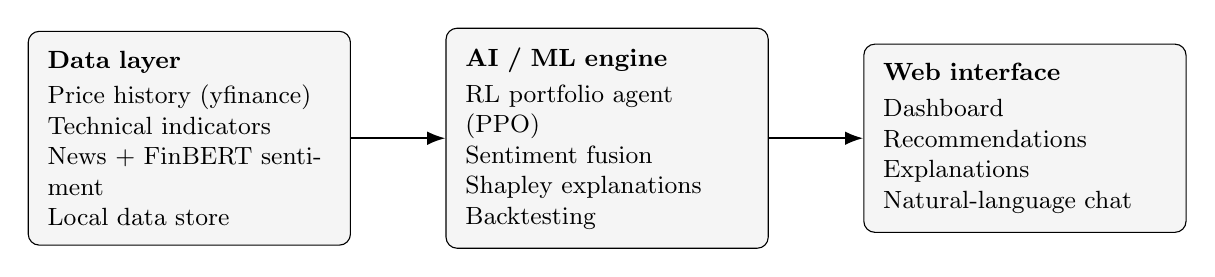
\begin{tikzpicture}[every node/.style={font=\small}]
\tikzset{tier/.style={draw, rounded corners, align=left, text width=3.6cm,
  fill=black!4, inner sep=7pt}}
\node[tier] (data) {\textbf{Data layer}\\[2pt]
  Price history (yfinance)\\ Technical indicators\\ News + FinBERT sentiment\\ Local data store};
\node[tier, right=12mm of data] (engine) {\textbf{AI / ML engine}\\[2pt]
  RL portfolio agent (PPO)\\ Sentiment fusion\\ Shapley explanations\\ Backtesting};
\node[tier, right=12mm of engine] (web) {\textbf{Web interface}\\[2pt]
  Dashboard\\ Recommendations\\ Explanations\\ Natural-language chat};
\draw[-{Latex}, thick] (data) -- (engine);
\draw[-{Latex}, thick] (engine) -- (web);
\end{tikzpicture}
\caption{The three-tier design. Market data is prepared on the left. The engine
decides and explains in the middle. The interface presents results on the right.}
\label{fig:arch}
\end{figure}

\subsection{Data layer}

The data layer fetches daily price history for the chosen assets through the
yfinance API and caches it on disk. A run then repeats exactly and does not depend
on the network each time. If the source is down it falls back to a simulated price
series, which keeps development and demos working offline. From the raw prices it
builds a small set of technical features per asset: short and medium return, a
relative strength index, a MACD trend measure, recent volatility and two
moving-average ratios. These cover the three signal types traders rely on: momentum,
mean reversion and trend. Each feature is scaled to a similar range so no single one
dominates the input to the network. The same layer holds the news pipeline.
Headlines are scored by FinBERT. That score becomes one more feature the agent can
read, which is how the text signal enters the decision.

The choices in this layer are deliberate. I use daily data rather than intraday,
because the target user is not a day trader and daily prices are clean and free to
get. That keeps the project reproducible. The features are kept few and standard, so
each one has a clear meaning the explanation can point to. Adding dozens of
indicators would lift accuracy slightly at best, while making the reasons harder to
read. Scaling every feature to a similar range stops a large-valued input from
dominating the network early in training. These are small decisions. Together they
keep the data honest and the later explanations legible.

\subsection{Decision engine}

The engine treats portfolio management as a Markov decision process, in the style of
Jiang et al.\ \cite{jiang2017}. At the close of each day the agent sees the feature
vector for every asset plus its current weights. The current weights are there on
purpose, so the agent knows where it already stands and can avoid needless trading.
It outputs a target weight for each asset and for cash. A concentration cap limits
how much can go into any one asset. That keeps the portfolio diversified and stops
the agent making one large bet that happens to pay off in the test period. The agent
is trained with Proximal Policy Optimisation \cite{schulman2017}, a stable
policy-gradient method that handles the continuous weight output well and is less
fiddly to tune than value-based methods. The reward is the daily log return after
transaction costs, with small penalties for risk and for turnover. The penalties
matter. Without the turnover penalty the agent churns the portfolio and trading
costs wipe out the gains. Without the risk term it chases volatile assets. The
reward is the main design lever. Section 4 shows how changing it changed the
behaviour.

The action is continuous, since a weight can take any value between zero and the
cap. A value-based method like the deep Q-network of Mnih et al.\ \cite{mnih2015}
picks from a fixed set of actions, so it does not fit well here. PPO works directly
with continuous outputs and trains steadily without much tuning, which is why I
picked it. The state is kept small on purpose: a handful of features per asset plus
the current weights. A small state is easier to learn from on limited history. It
also keeps the later explanation readable, since there are only a few inputs to
trace a decision to.

\subsection{Explanation layer}

Every allocation is explained by tracing it back to the input features. I treat the
agent as a function from features to weights. Each feature gets a Shapley value that
says how much it moved the decision, using the sampling method of \v{S}trumbelj and
Kononenko \cite{strumbelj2014}. I chose Shapley attribution over LIME for two
reasons. It gives a local view of a single decision as well as a global view across
many decisions. Its contributions also add up to the output in a way that is easy to
present. The result is a ranked list of drivers for each holding. A short template
then turns the top drivers into a sentence a non-expert can read, for example that
an asset was favoured because its trend and momentum were strong. In the full system
a local language model writes this text. The template is the stand-in for now. It
keeps the wording tied to the attribution rather than free-form.

\subsection{Web interface}

The interface is a single-page dashboard. It shows the portfolio value over time
against a buy-and-hold line, the current split across assets and how that split has
changed. A recommendations view lists each holding with its target weight. The user
can open a panel on any holding to see why it was chosen. A chat view answers plain
questions about the portfolio, such as why one asset was favoured over another. The
flow is short: set up a portfolio, read the recommendation, open the reason if you
want it, ask a question if you are still unsure. Someone with no finance or coding
background should be able to follow it without instructions.

A few choices support that. The wording avoids jargon, so a recommendation reads as
a plain sentence rather than a set of ratios. Gains and losses use colour and
direction, not just numbers, so the state of the portfolio is clear at a glance. The
most important figures sit at the top. The detail behind a decision stays hidden
until the user asks for it, which keeps the first view simple. The aim is to lower
the same trust barrier the literature describes, by making both the advice and the
reason easy to take in.

I built a working version of this interface as a dashboard, fed with the real output
of the prototype agent, to check that the design holds up. It is a multi-screen
application, not a single page. Figure~\ref{fig:ui-dashboard} shows the main
dashboard. Figure~\ref{fig:ui-screens} shows the other four screens: recommendations
with their reasons, the global explanation view, a natural-language assistant and a
performance view. Live market data, the FinBERT signal and a language-model chat are
still to come in the full build. The layout and the explanation flow are already in
place.

\begin{figure}[H]
\centering
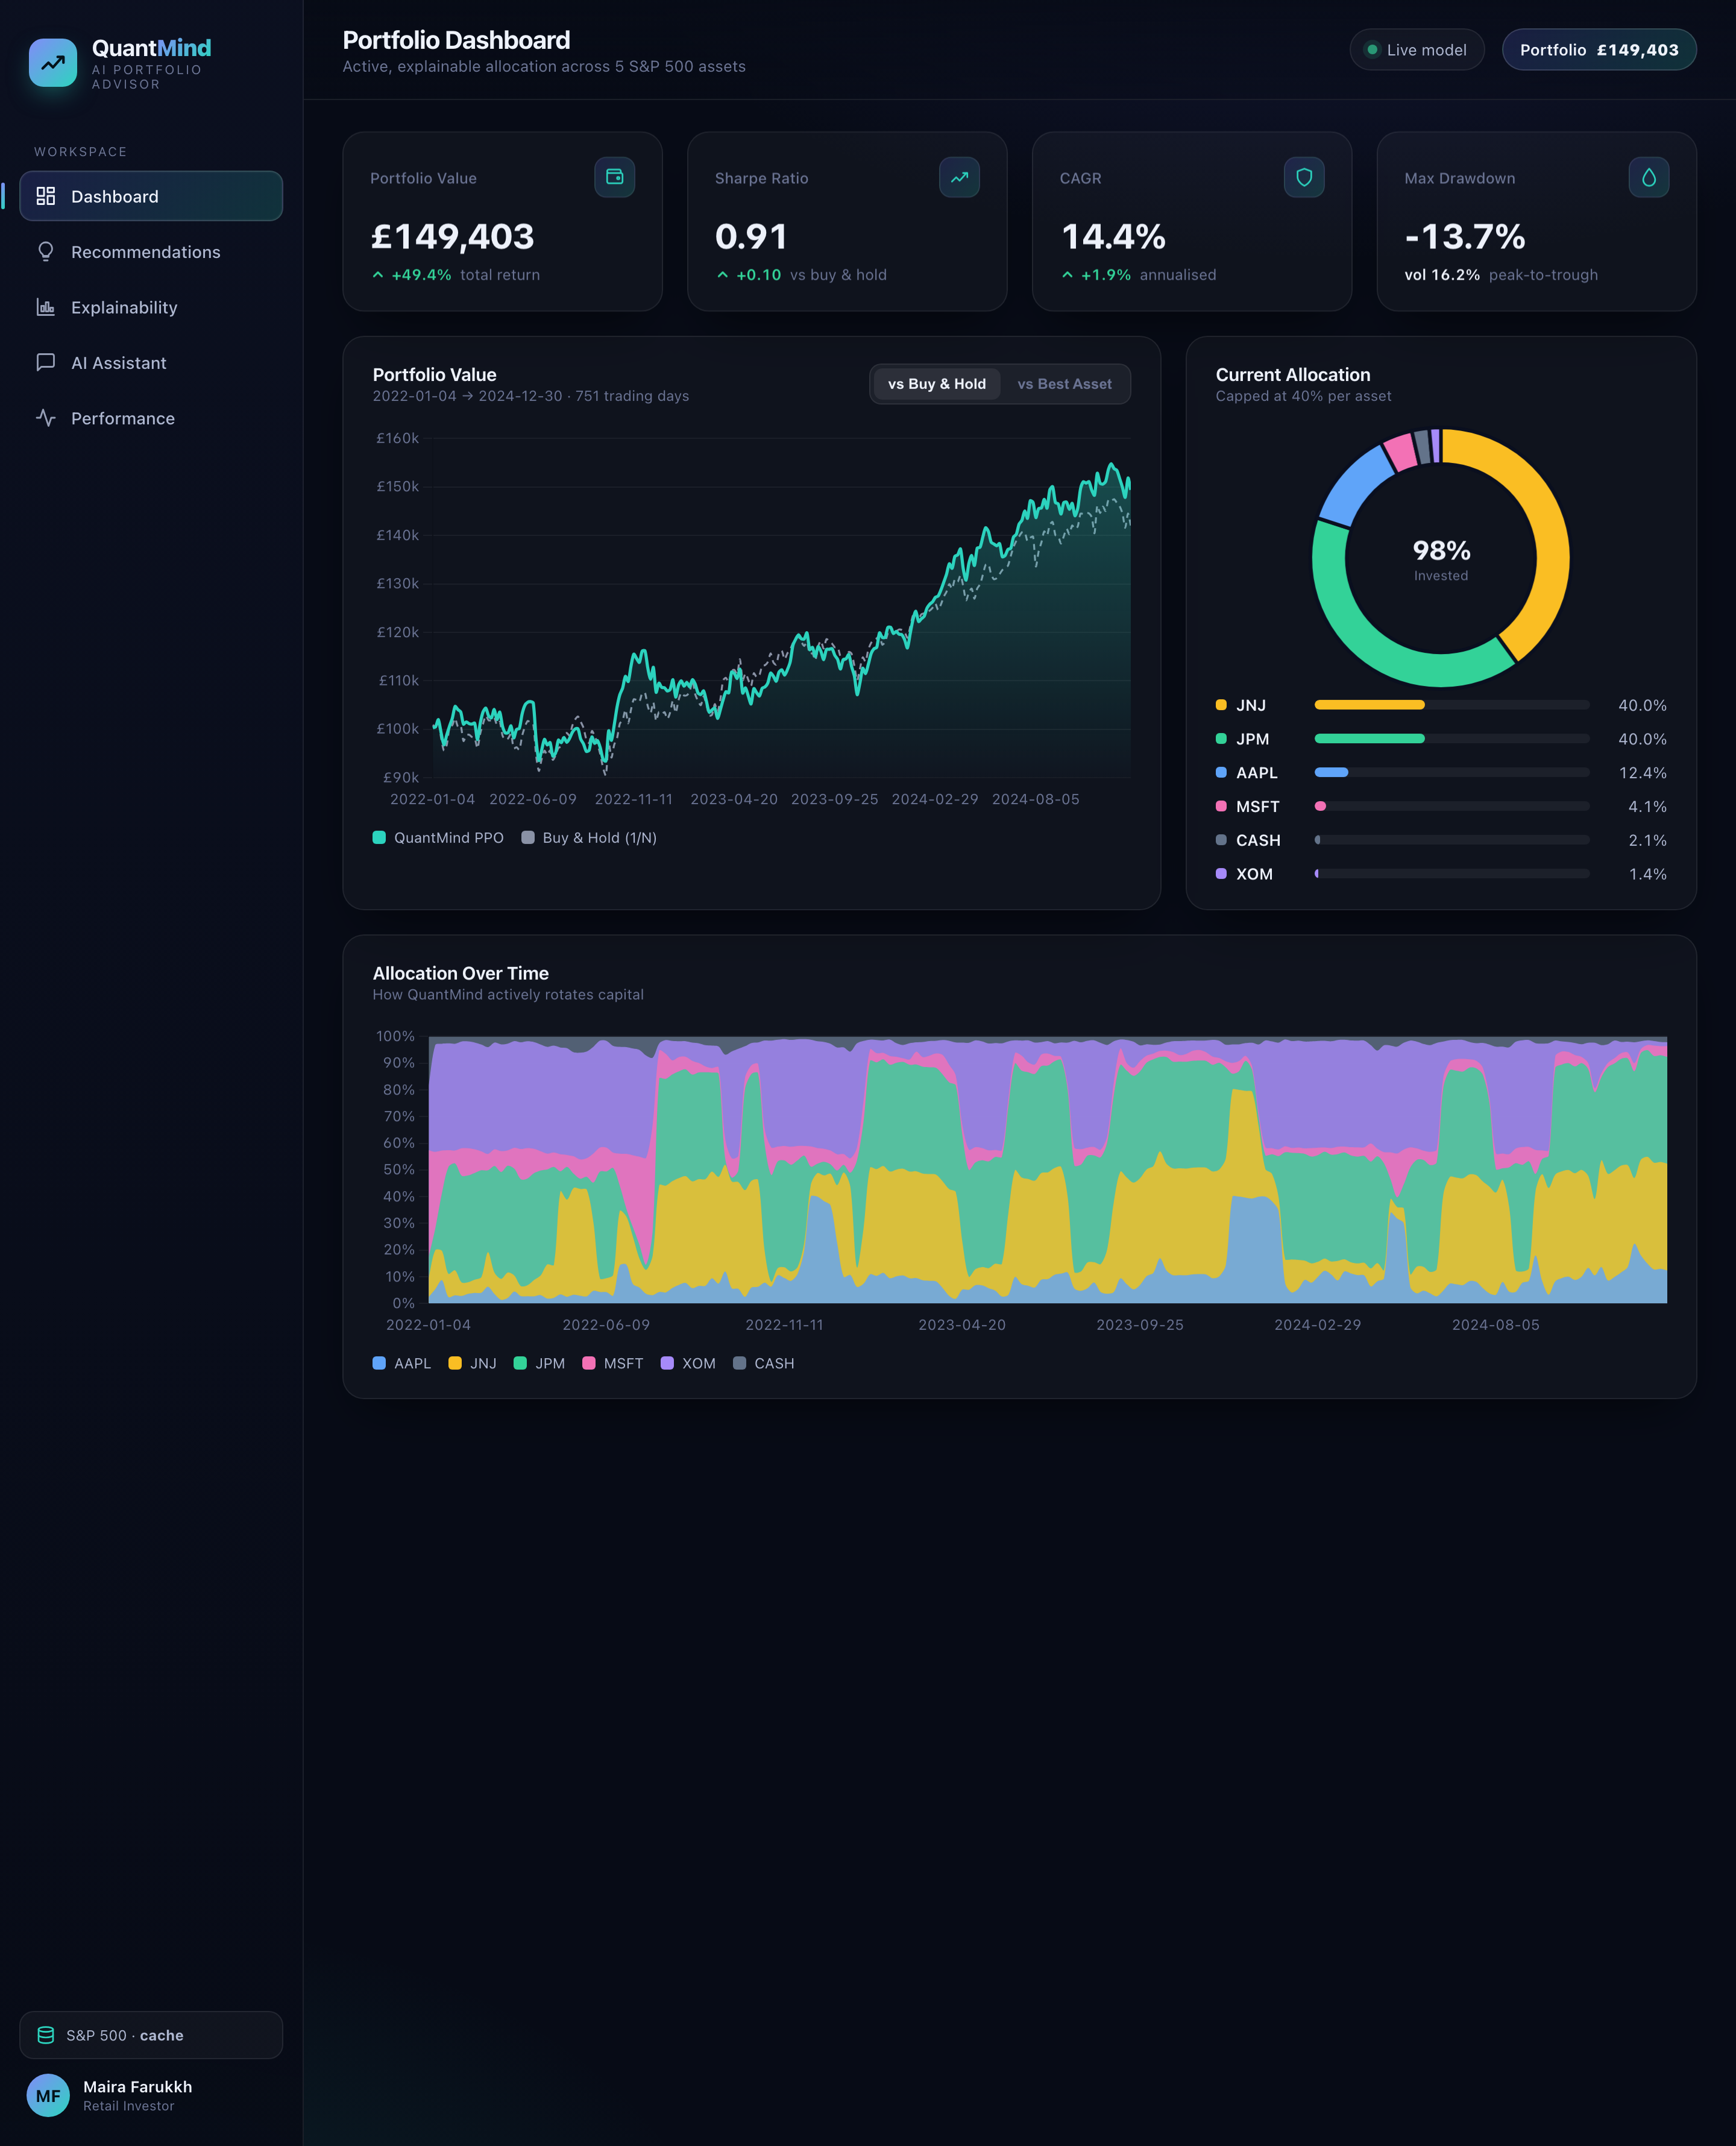
\includegraphics[width=0.95\textwidth]{figures/ui_dashboard.png}
\caption{The QuantMind dashboard: portfolio value against a buy-and-hold line, the
current allocation, plus how the mix changes over time.}
\label{fig:ui-dashboard}
\end{figure}

\begin{figure}[H]
\centering
\begin{minipage}{0.49\textwidth}\centering
  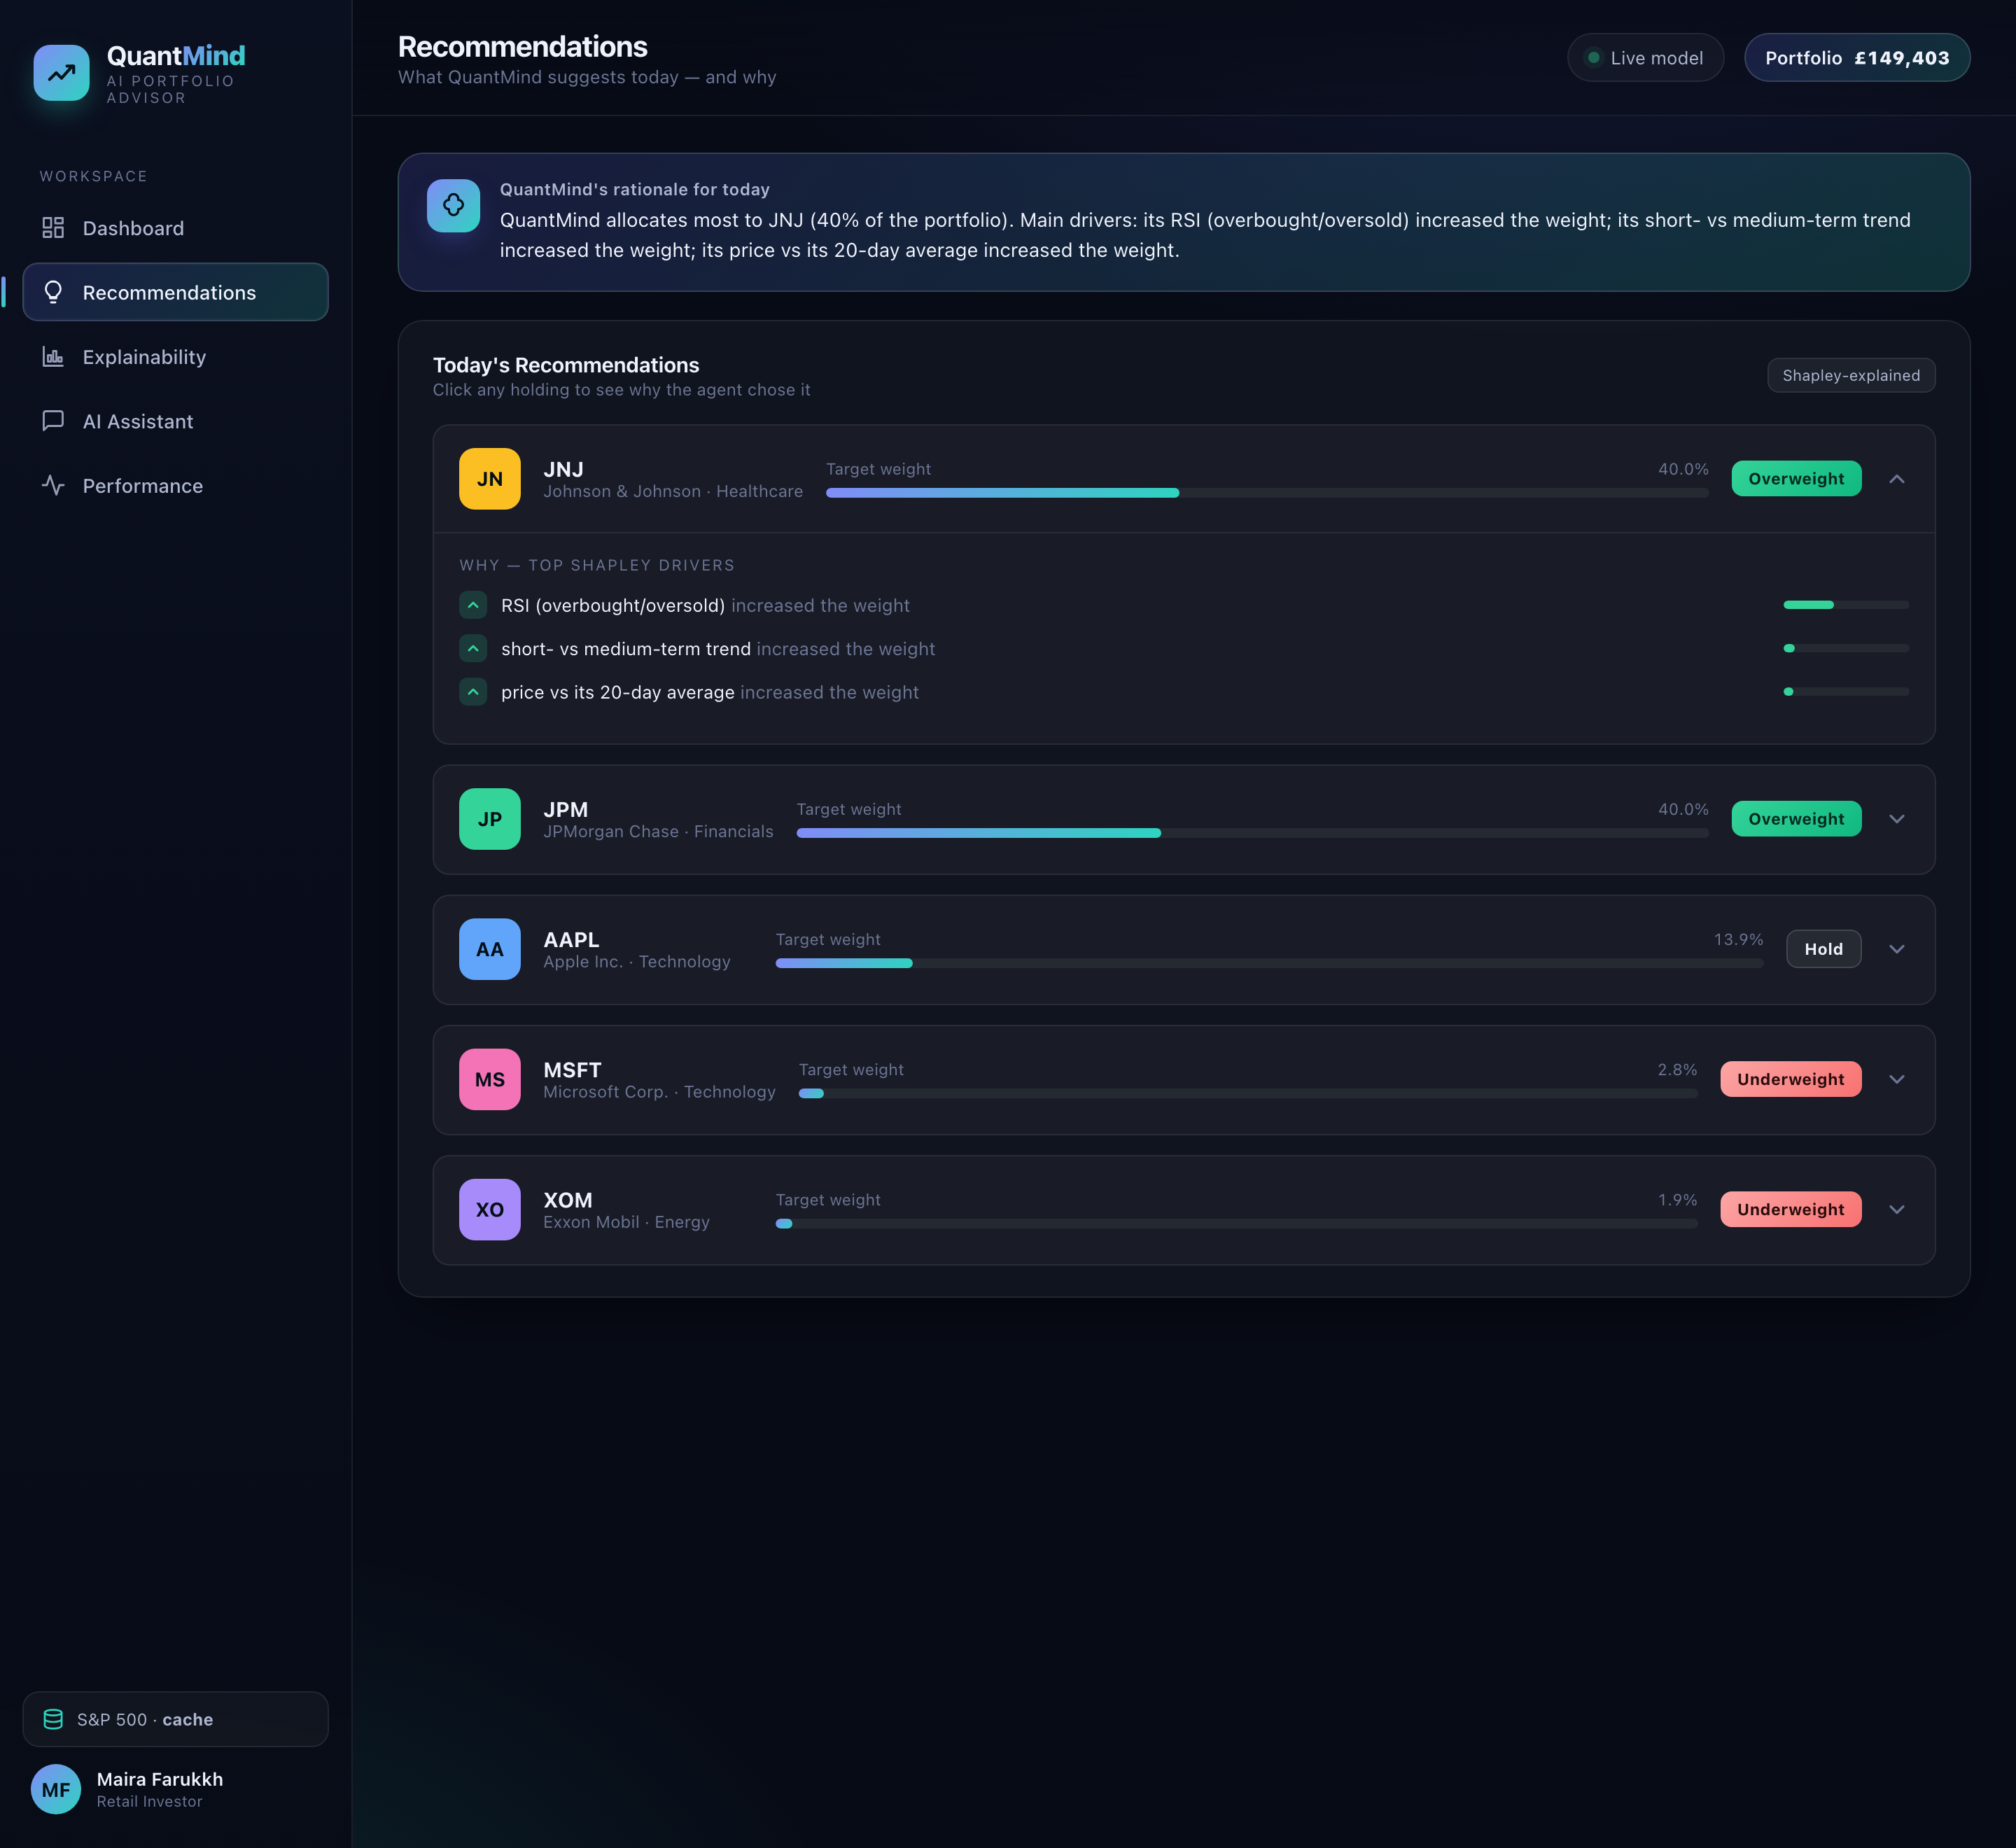
\includegraphics[width=\linewidth]{figures/ui_recommendations.png}\\
  {\small (a) Recommendations, with the reasons for the top holding}
\end{minipage}\hfill
\begin{minipage}{0.49\textwidth}\centering
  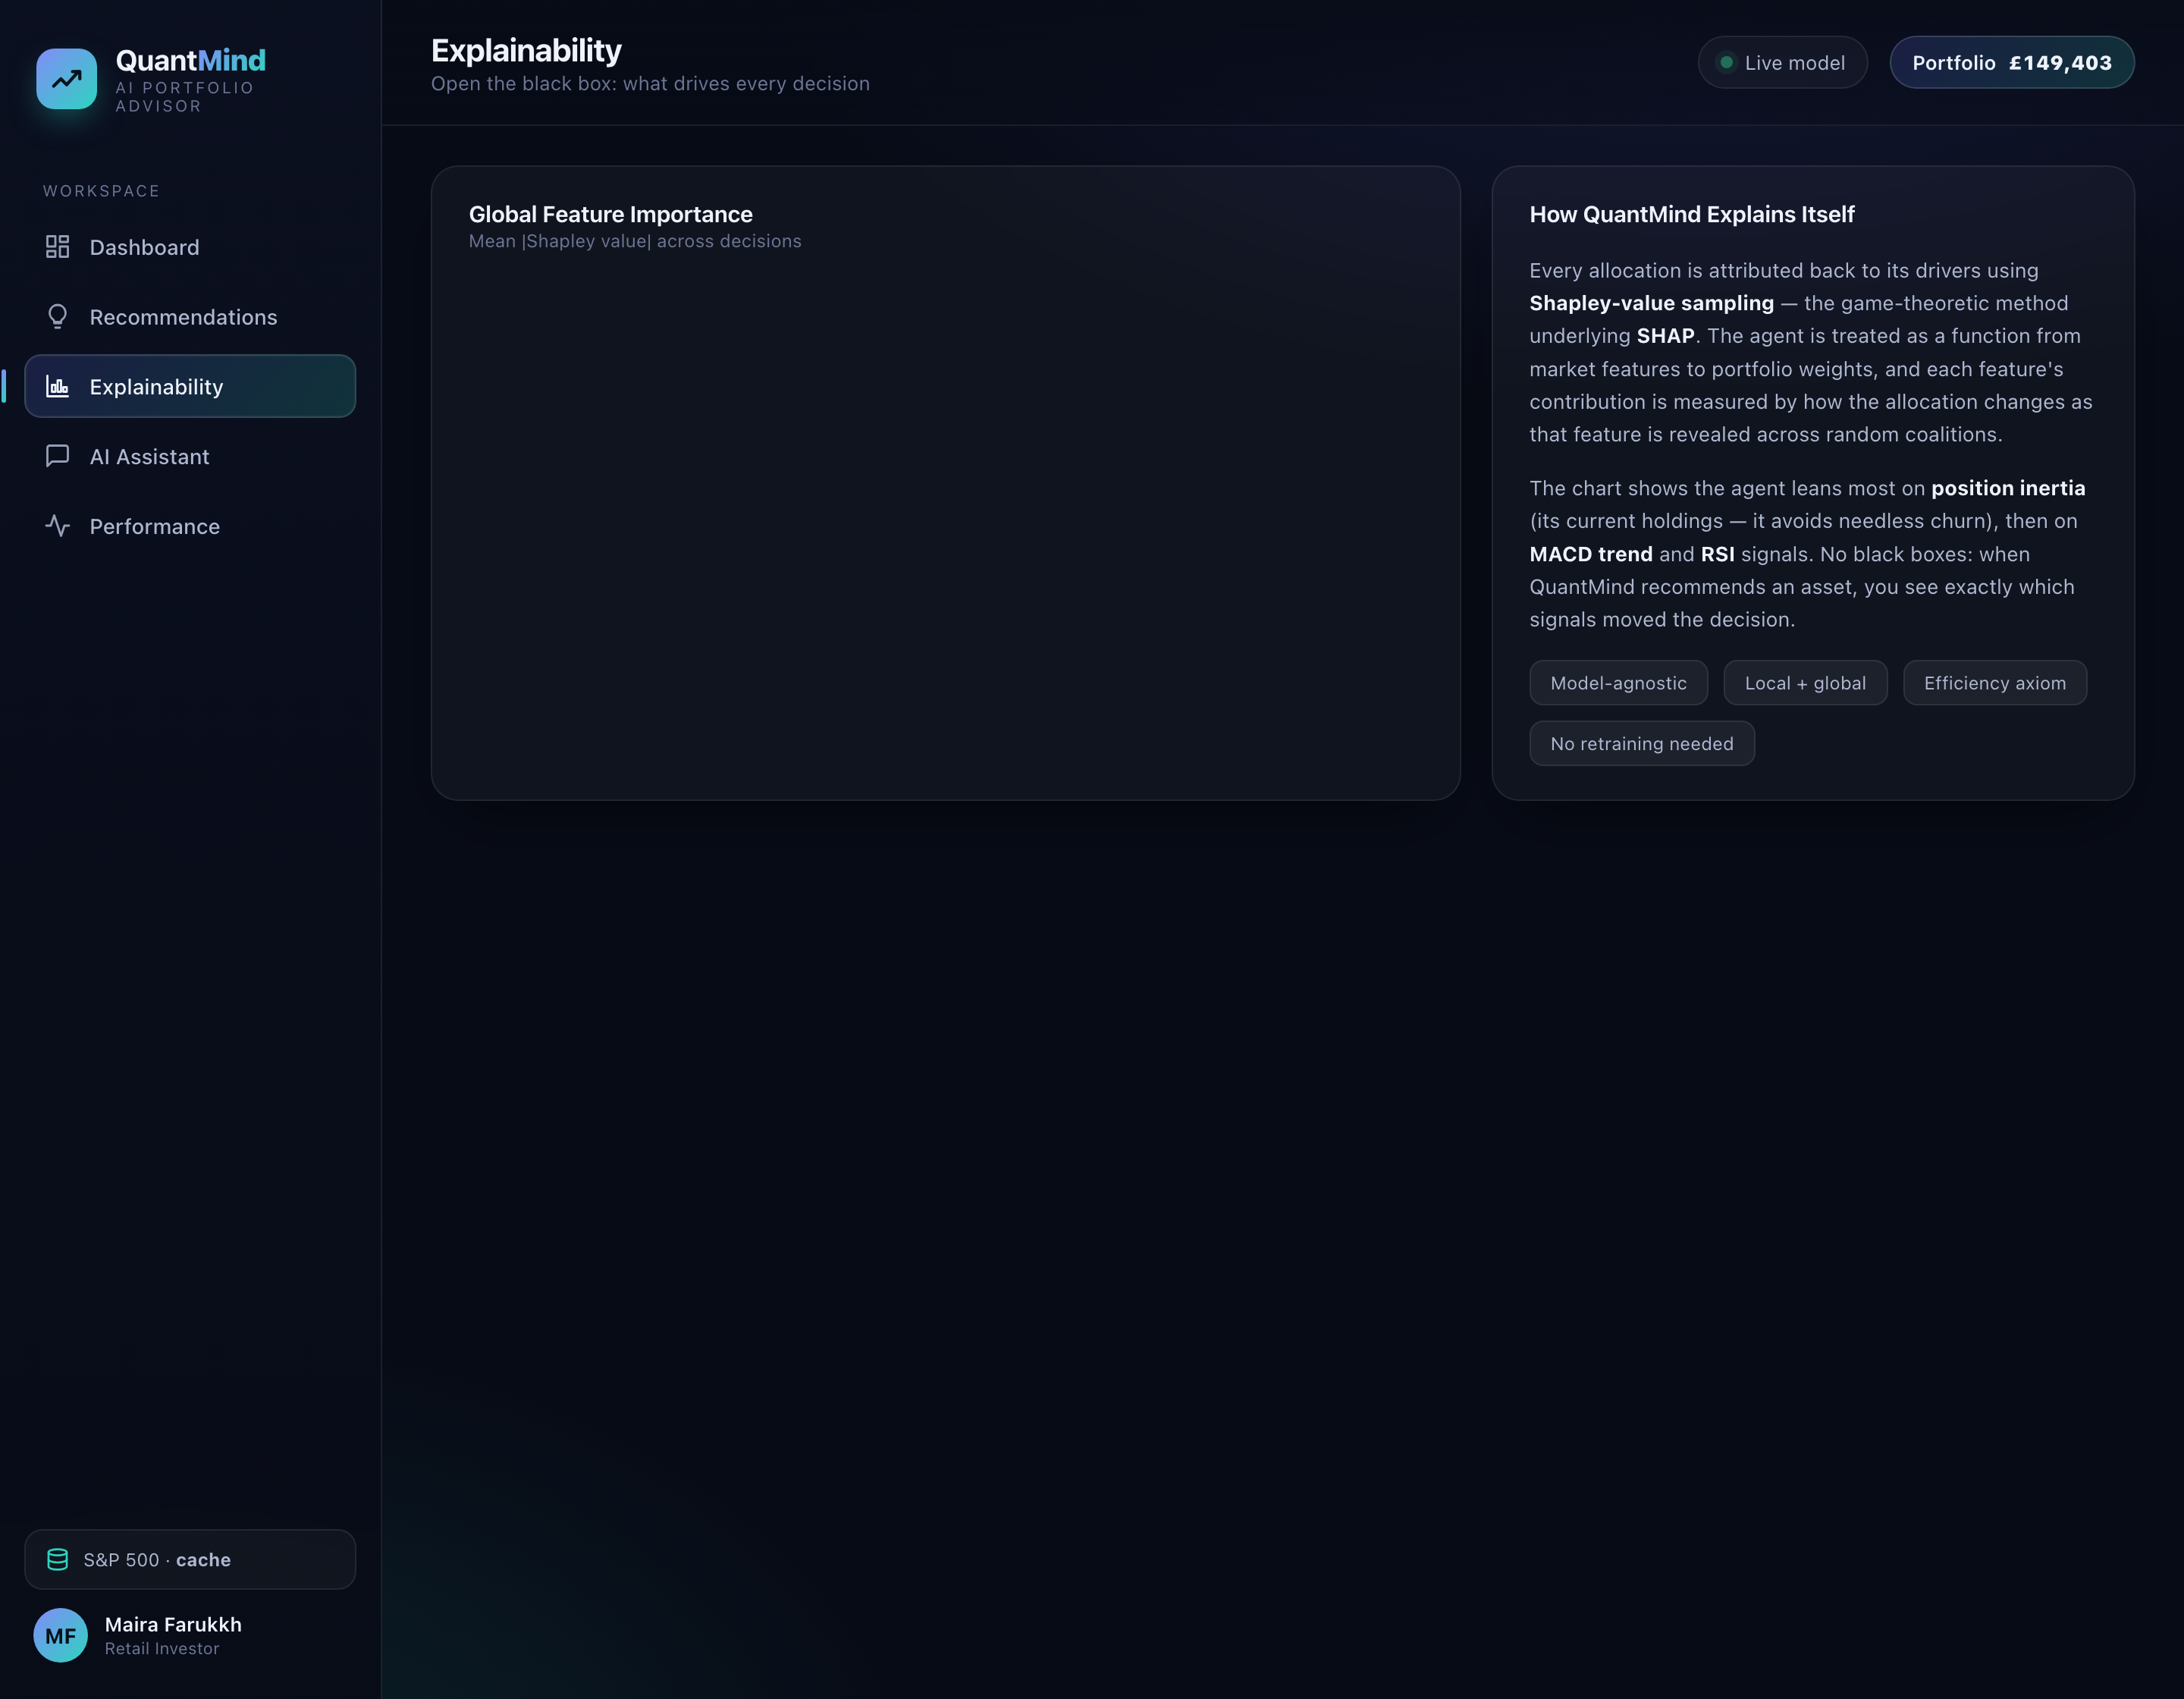
\includegraphics[width=\linewidth]{figures/ui_explainability.png}\\
  {\small (b) Explainability: global feature importance}
\end{minipage}

\vspace{8pt}
\begin{minipage}{0.49\textwidth}\centering
  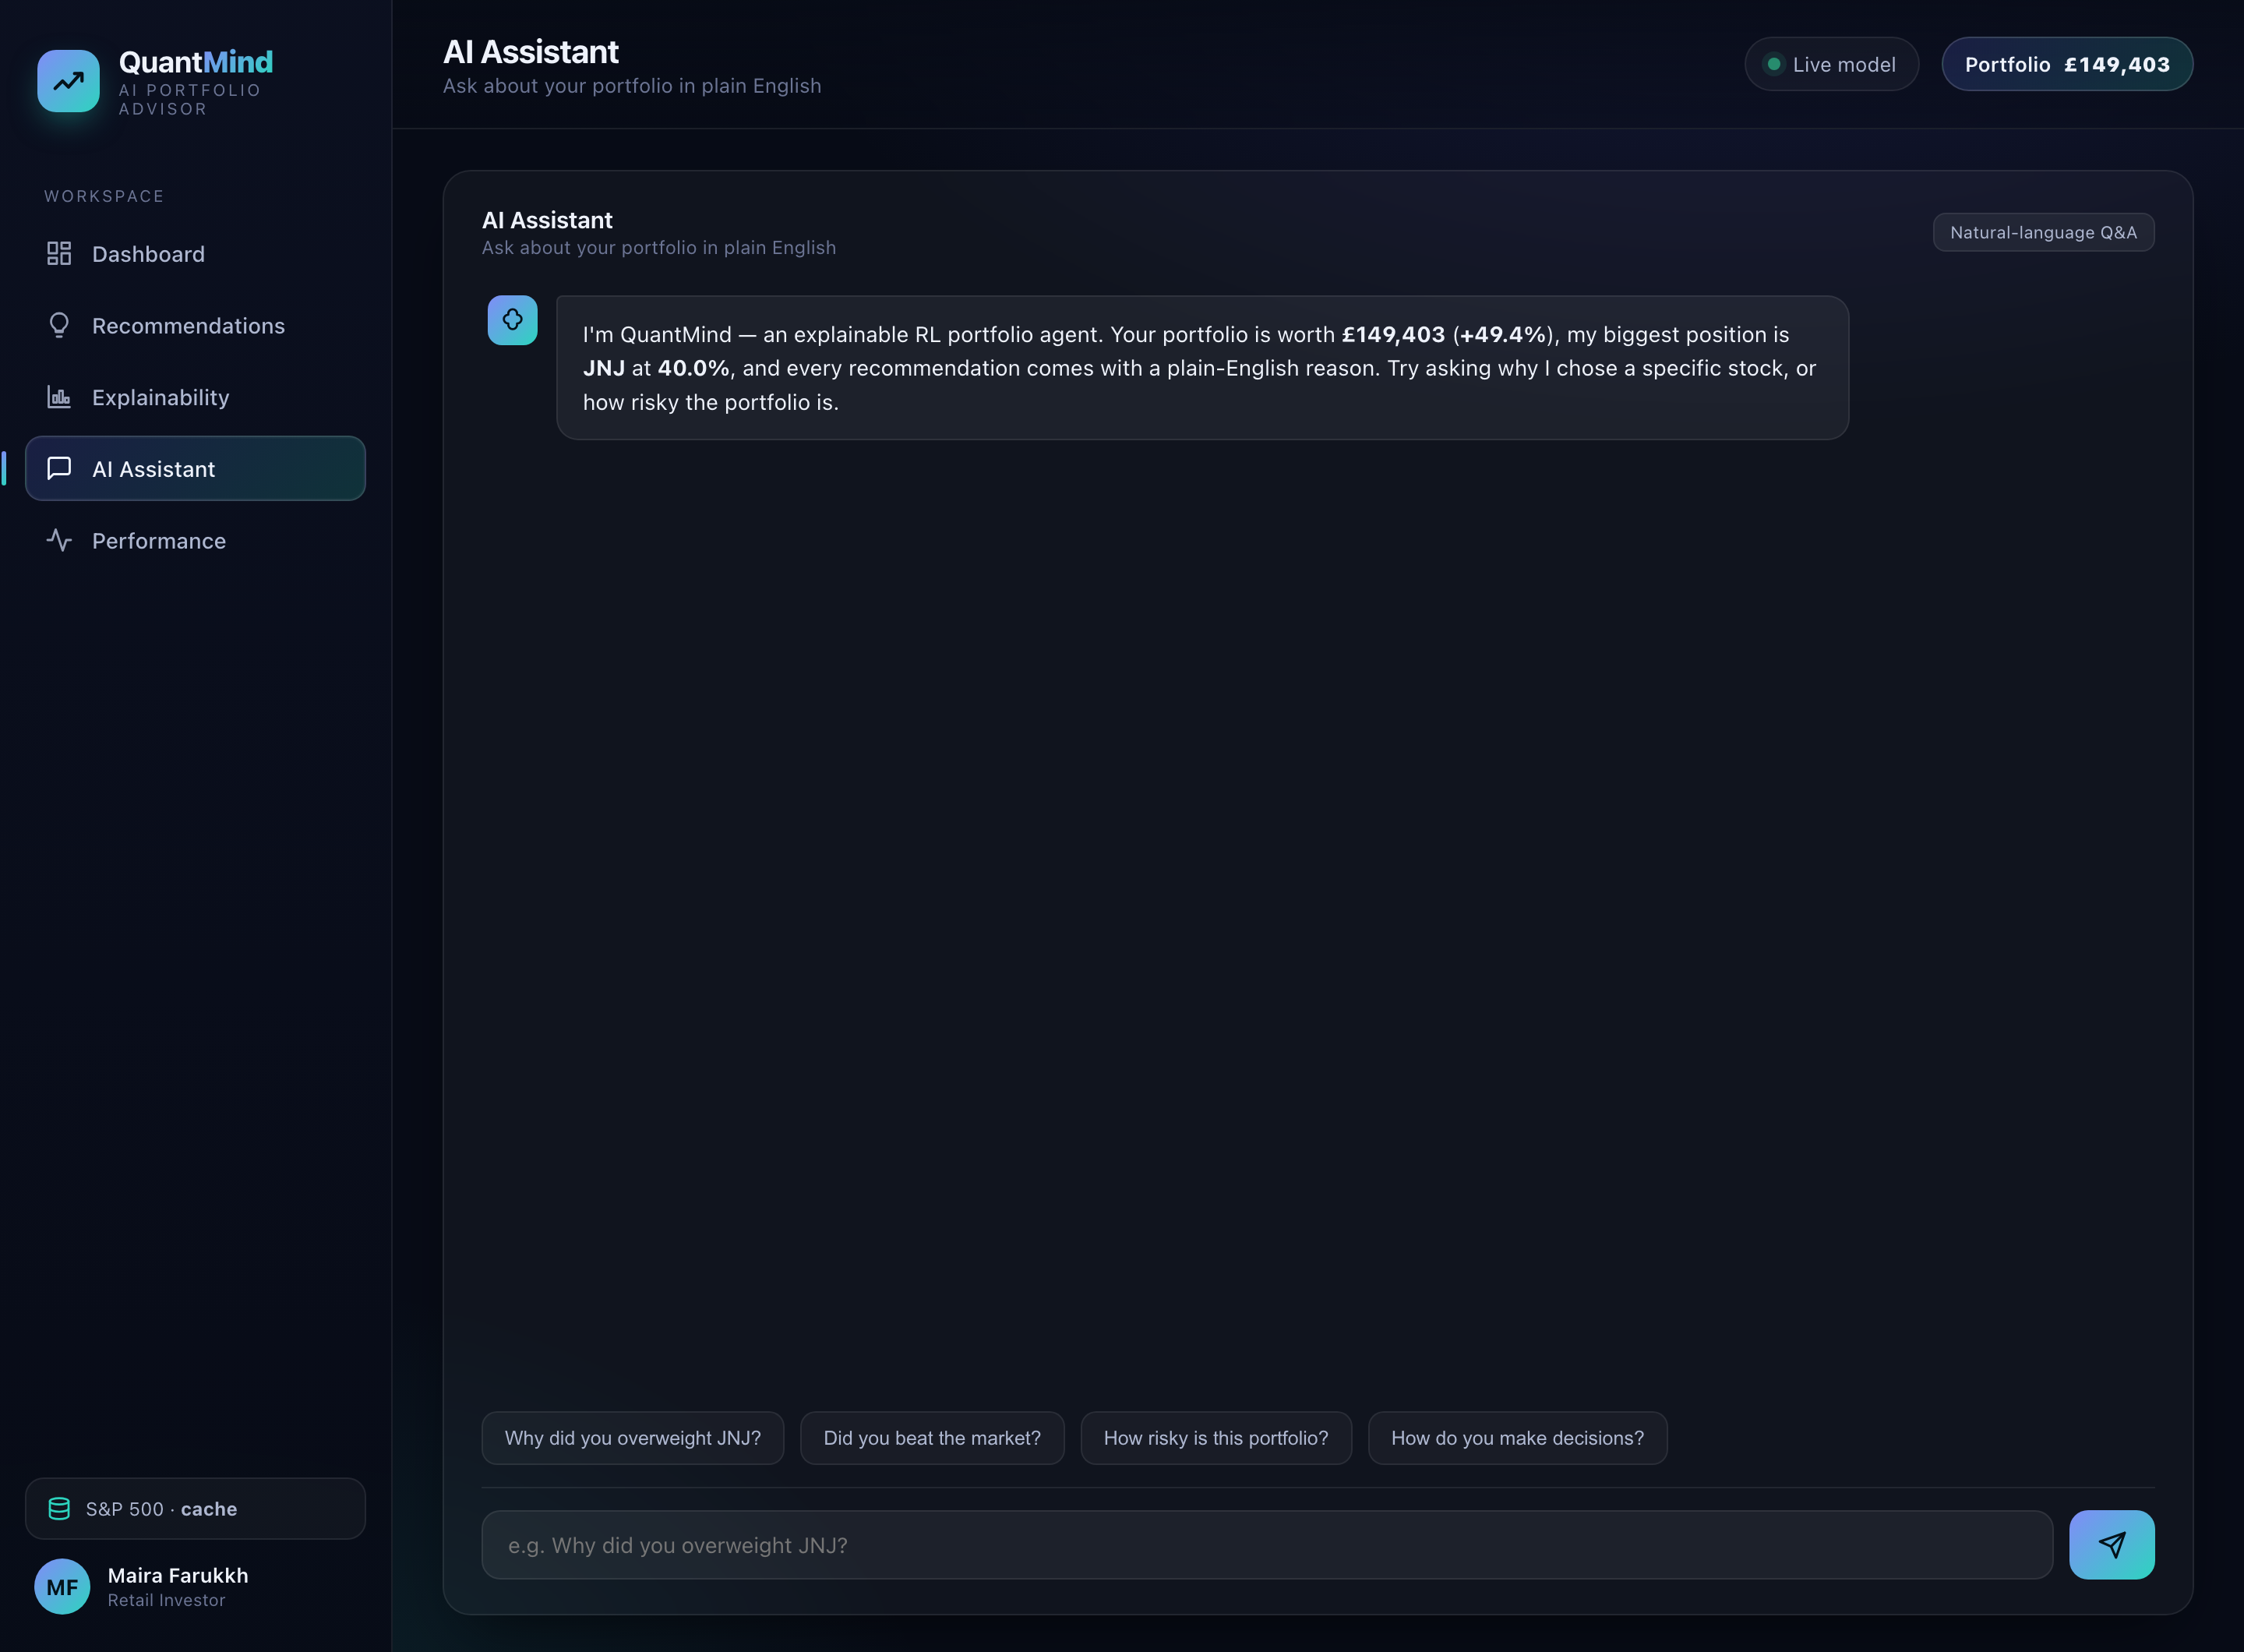
\includegraphics[width=\linewidth]{figures/ui_assistant.png}\\
  {\small (c) Natural-language assistant}
\end{minipage}\hfill
\begin{minipage}{0.49\textwidth}\centering
  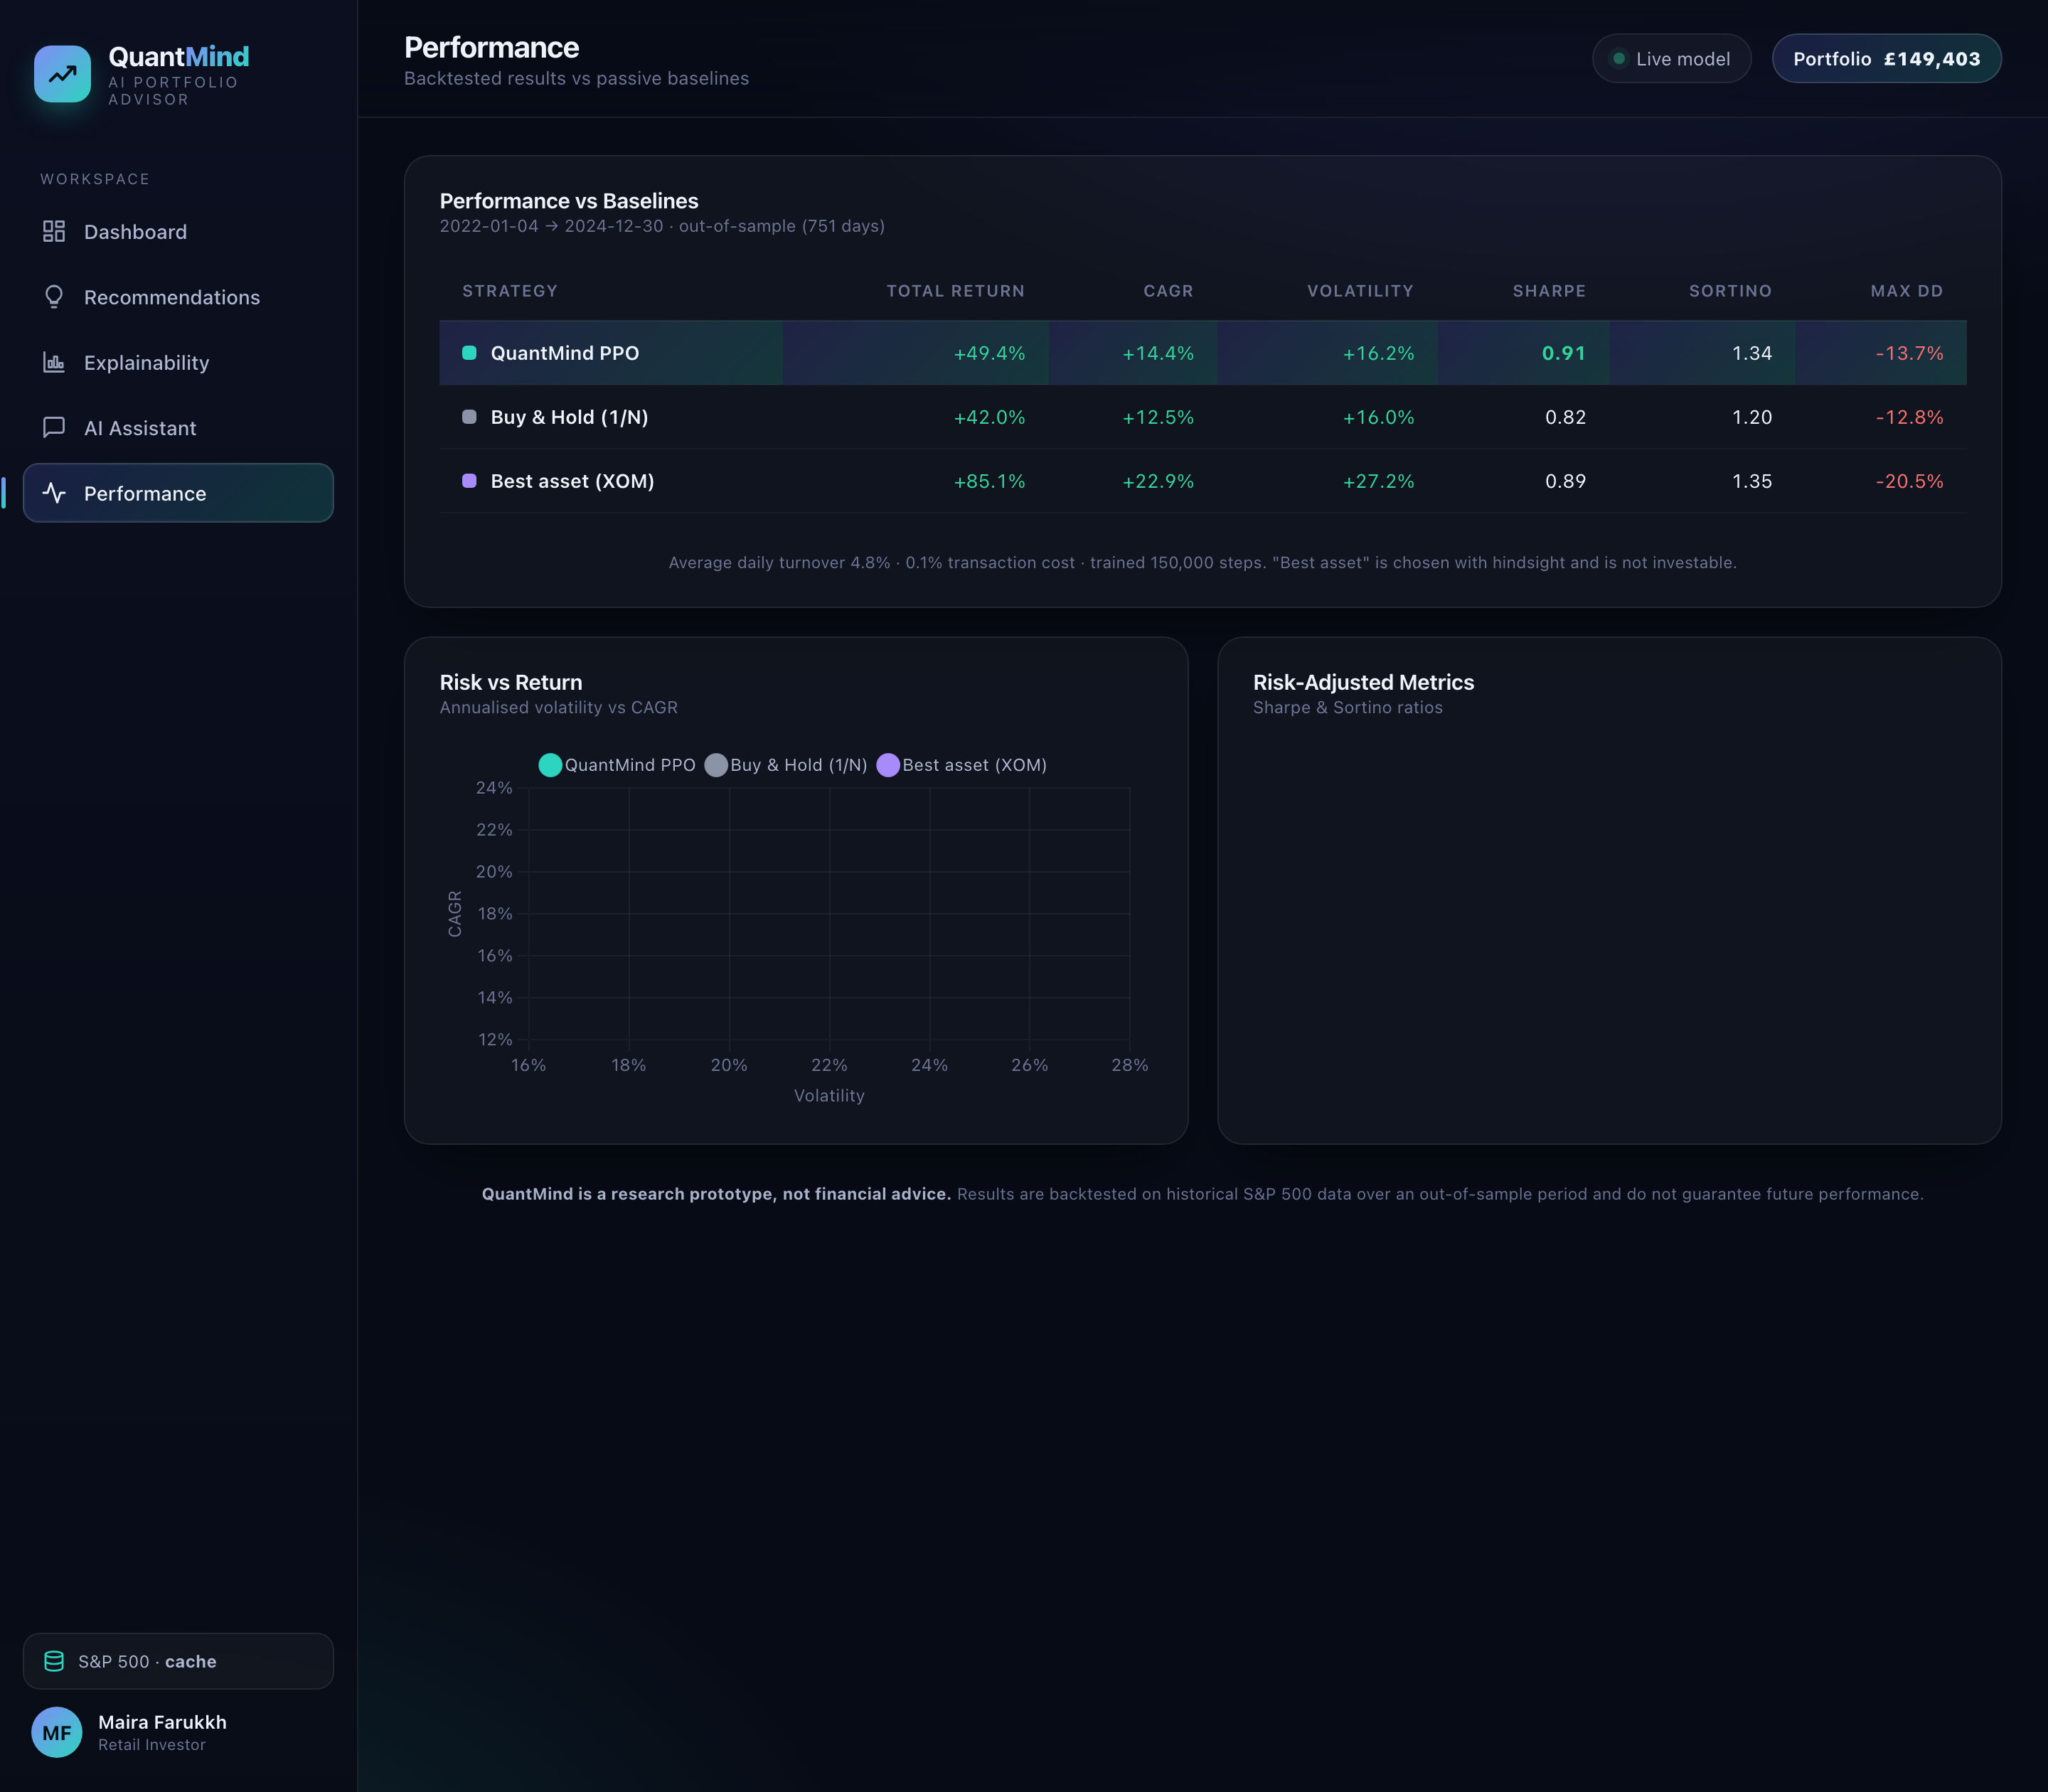
\includegraphics[width=\linewidth]{figures/ui_performance.png}\\
  {\small (d) Performance against baselines}
\end{minipage}
\caption{The other four screens of the web interface. The site is a multi-screen
dashboard rather than one page.}
\label{fig:ui-screens}
\end{figure}

\subsection{Workplan}

The project runs in four phases over about six months. Table~\ref{tab:plan} lists
them with their main outputs and the main risk in each. Every phase ends with
something that works, so a later slip does not leave the project with nothing to
show. The full build is the largest phase, so it carries the most slack. I integrate
parts one at a time rather than all at once, which makes faults easier to find. The
user study in phase four is the part most exposed to delay, since it depends on
other people. So recruitment starts early. The target is kept to a size I can
realistically reach.

\begin{table}[H]
\centering
\caption{Workplan with deliverables and the main risk per phase.}
\label{tab:plan}
\begin{tabular}{p{2.4cm} p{1.6cm} p{4.0cm} p{4.0cm}}
\toprule
Phase & Weeks & Deliverable & Main risk and response \\
\midrule
1. Research & 1--3 & Literature review, problem framing & Scope too wide; fix the asset universe early. \\
2. Design + RL prototype & 4--8 & Working agent, backtest, explanations & Data leakage; check timing, hold out a test set. \\
3. Full build & 9--18 & Sentiment fusion, language model, web app & Largest phase; keep slack, integrate in stages. \\
4. Evaluation + write-up & 19--24 & User study, final report & Recruiting users; start early, keep $n \geq 15$. \\
\bottomrule
\end{tabular}
\end{table}

\subsection{Evaluation strategy}

The project has two kinds of aim, financial and human. So it needs two kinds of
test. The template suggests evaluating the advice the bot gives. This plan builds on
that and says how.

For the agent, the test is a backtest on data it never trained on. The split is by
date: the earlier years train the agent, the most recent years are held out. I
report total return, compound annual growth rate, annualised volatility, the Sharpe
\cite{sharpe1966} and Sortino \cite{sortino1994} ratios and maximum drawdown. I
compare against an equal-weight buy-and-hold baseline and against the best single
asset chosen with hindsight. Sharpe is the headline, because the goal is
risk-adjusted return rather than raw profit. Sortino and drawdown check the
downside, which is what a cautious user cares about. Turnover checks whether returns
survive trading costs. A single split can flatter a model by luck. So I plan
walk-forward testing across several windows, repeated runs with different random
seeds, plus an ablation that turns the sentiment feature on and off to see whether it
really helps.

For the human aims, a backtest is not enough. The point is that people understand
and trust the advice. I plan a small user study with at least fifteen non-expert
participants. They complete set tasks, such as creating a portfolio and reading a
recommendation, which gives a task-completion rate. They fill in the System
Usability Scale for the interface, a standard and comparable measure. They also
answer a short questionnaire on whether the explanations made them more confident in
the advice. This second part connects to the trust findings of Meske et al.\
\cite{meske2022}. It tests the central claim of the project head-on: that explaining
a decision makes a non-expert more willing to act on it.

To keep the user study honest, I test the trust question with two versions of the
interface: one that shows the explanations, one that hides them. Any difference can
then be put down to the explanations rather than the tool in general. Participants
give informed consent. No real money is involved. Results are reported as group
figures, with no personal data kept. The sample is small, so the study is there to
show direction and surface usability problems, not to prove a statistical effect. A
larger study would follow if the direction looks positive. Put together, the
backtest checks whether the advice is any good. The user study checks whether people
can use and trust it. The project needs both to claim success.

%%%%%%%%%%%%%%%%%%%%%%%%%%%%%%%%%%%%%%%%%%%%%%%%%%%%%%%%%%%%%%%%%%%%%%%%%%%%%%%%
% 4. FEATURE PROTOTYPE
%%%%%%%%%%%%%%%%%%%%%%%%%%%%%%%%%%%%%%%%%%%%%%%%%%%%%%%%%%%%%%%%%%%%%%%%%%%%%%%%
\section{Feature Prototype}

\subsection{What I built and why}

The hardest part of QuantMind is the decision engine: the agent that turns market
data into an allocation, plus the layer that explains it. The other parts, such as
the data feeds and the web pages, are more standard. So the prototype is the agent
and its explanation, built end to end on real market data. It leaves out the
sentiment model, the language model and the full web app. Those belong to the final
build. The point is to show the difficult part works and to flush out the problems
early.

\subsection{Data and features}

I used daily prices for five S\&P~500 companies from different sectors: Apple,
Microsoft, JPMorgan, Exxon Mobil and Johnson \& Johnson. One name from each of five
sectors keeps the portfolio diversified and the explanations readable, since there
are not many inputs to reason about. The data comes from yfinance \cite{yfinance}
and covers 2015 to 2024, which is 2{,}515 trading days, cached locally. For each
asset I compute seven features: one- and five-day returns, a relative strength
index, a MACD trend measure, twenty-day volatility and two moving-average ratios.
The split is by date. The years 2015 to 2021 train the agent. The years 2022 to 2024
are held out for testing. That window includes the 2022 fall and the recovery after
it, so it is a fair test rather than a calm stretch picked to flatter the result.

\subsection{The agent}

I wrote a custom environment on the Gymnasium interface that frames the task as a
Markov decision process, following Jiang et al.\ \cite{jiang2017}. Each day the agent
sees the seven features for all five assets plus its current six weights. It then
outputs a target weight for each asset and for cash through a softmax. A 40\% cap
limits any single name, with the excess spread across the others. The reward is the
daily log return after a 0.1\% transaction cost, with a penalty on volatility and a
penalty on turnover:
\begin{equation}
r_t = \log\!\left(1 + R^{\text{net}}_t\right) - \lambda_{\text{risk}}\,\sigma_t
      - \lambda_{\text{turn}}\,\tau_t .
\label{eq:reward}
\end{equation}
Here $R^{\text{net}}_t$ is the return after costs, $\sigma_t$ is recent volatility
and $\tau_t$ is turnover. The agent is trained with Proximal Policy Optimisation
\cite{schulman2017} from the Stable-Baselines3 library \cite{sb3} for 150{,}000
steps, with a two-layer network of 128 units and a fixed random seed so the run
repeats. Training takes a couple of minutes on a laptop CPU, which keeps the loop
short enough to try changes quickly. To rule out the look-ahead problem described
below, I checked that a decision made at the close of one day is only ever rewarded
with the next day's return. Nothing the agent sees includes information from after
the choice.

\subsection{Explanations}

To explain a decision I treat the trained policy as a function from features to
weights, then give each feature a Shapley value by sampling \cite{strumbelj2014}.
This is the idea behind SHAP \cite{lundberg2017} and the local explanations of
Ribeiro et al.\ \cite{ribeiro2016}, but written from scratch in NumPy so the
prototype needs no extra libraries. Writing it myself also kept the method
transparent, since I could check each step against the definition. It produces a
global ranking of which features matter most. For any single day it lists the
drivers behind each holding, which a short template turns into a sentence.

\subsection{Results}

Table~\ref{tab:results} reports the held-out test period. The agent beats the
buy-and-hold baseline on the Sharpe ratio (0.91 against 0.82), on the Sortino ratio
and on total return, at about the same volatility. It also has a higher Sharpe than
the best single asset, while taking far less drawdown. The baselines earn the same
days the agent earns, so the comparison is fair. Average daily turnover is 4.8\%. The
agent trades, but it does not churn.

\begin{table}[H]
\centering
\caption{Performance on the held-out test period (2022--2024, 752 days).}
\label{tab:results}
\begin{tabular}{l c c c c c c}
\toprule
Strategy & Total ret. & CAGR & Vol. & Sharpe & Sortino & Max DD \\
\midrule
QuantMind PPO & 49.4\% & 14.4\% & 16.2\% & 0.91 & 1.34 & $-13.8\%$ \\
Buy \& Hold (1/N) & 42.0\% & 12.5\% & 16.0\% & 0.82 & 1.20 & $-12.8\%$ \\
Best asset (hindsight) & 85.1\% & 22.9\% & 27.2\% & 0.89 & 1.35 & $-20.5\%$ \\
\bottomrule
\end{tabular}
\end{table}

Figure~\ref{fig:equity} shows the portfolio value over the test period. The agent
stays above buy-and-hold for most of it. Figure~\ref{fig:alloc} shows the allocation
over time. The agent manages the portfolio rather than sit still. It holds more
energy (Exxon) during the 2022 inflation period, then rotates into financials and
healthcare later, always inside the 40\% cap. Figure~\ref{fig:shap} shows which
features drive its decisions. The biggest driver is the current holding, so the
agent prefers to stay put unless a signal is strong. After that come the MACD trend
and the relative strength index. That order is a useful check, because it matches the
turnover penalty in the reward: the agent has learned to value staying put.

\begin{figure}[H]
\centering
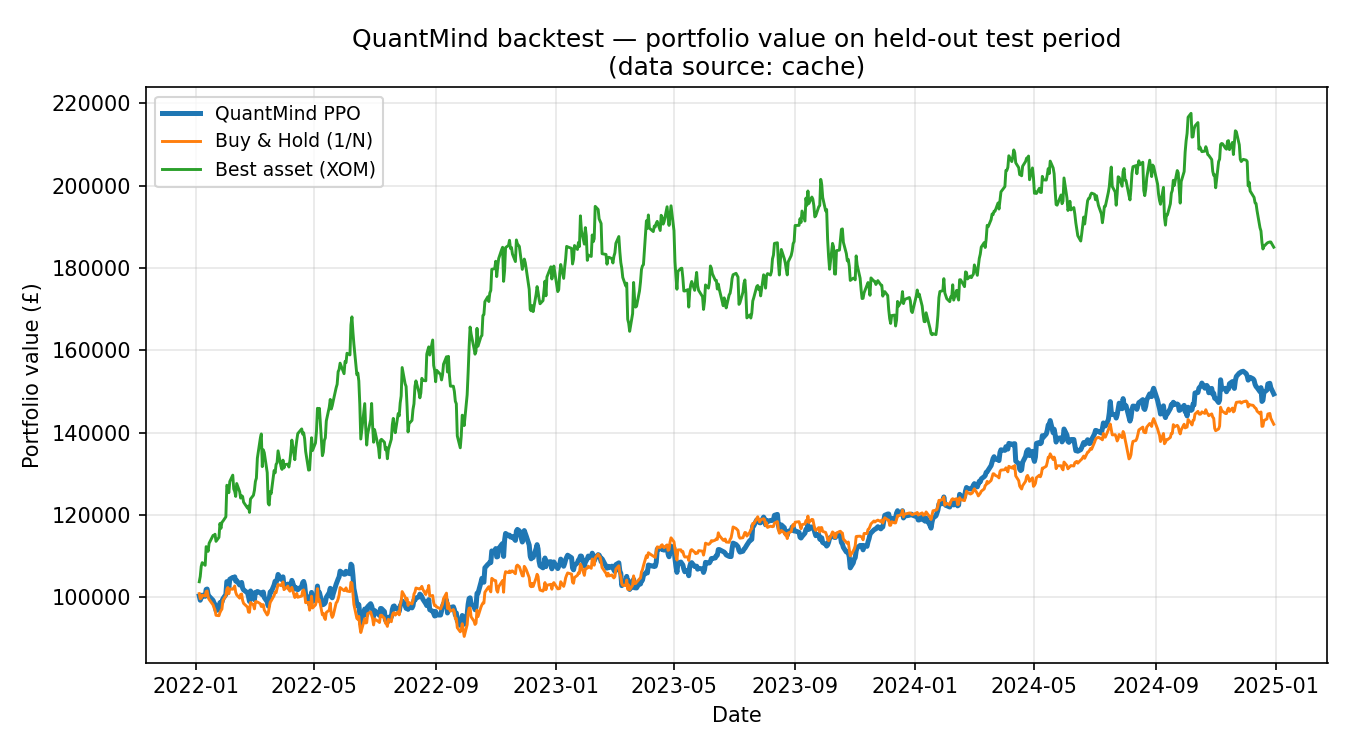
\includegraphics[width=0.85\textwidth]{figures/equity_curve.png}
\caption{Portfolio value on the held-out test period.}
\label{fig:equity}
\end{figure}

\begin{figure}[H]
\centering
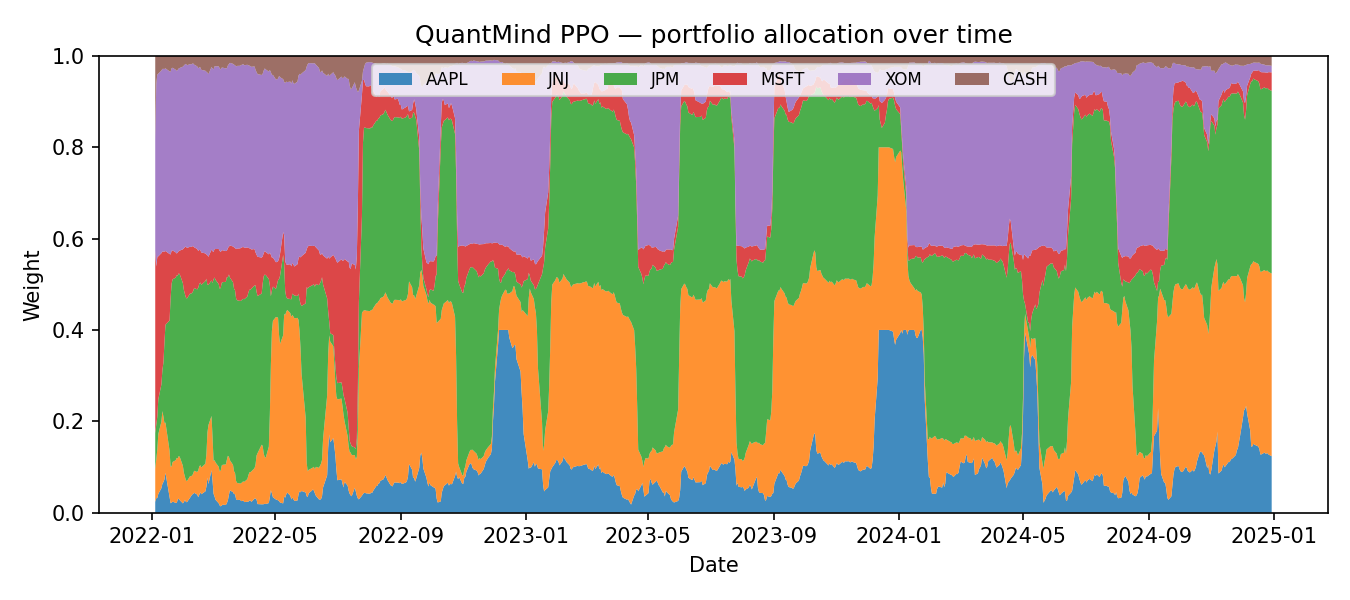
\includegraphics[width=0.85\textwidth]{figures/allocation.png}
\caption{Allocation over time. The mix changes with conditions and respects the 40\%
cap per asset.}
\label{fig:alloc}
\end{figure}

\begin{figure}[H]
\centering
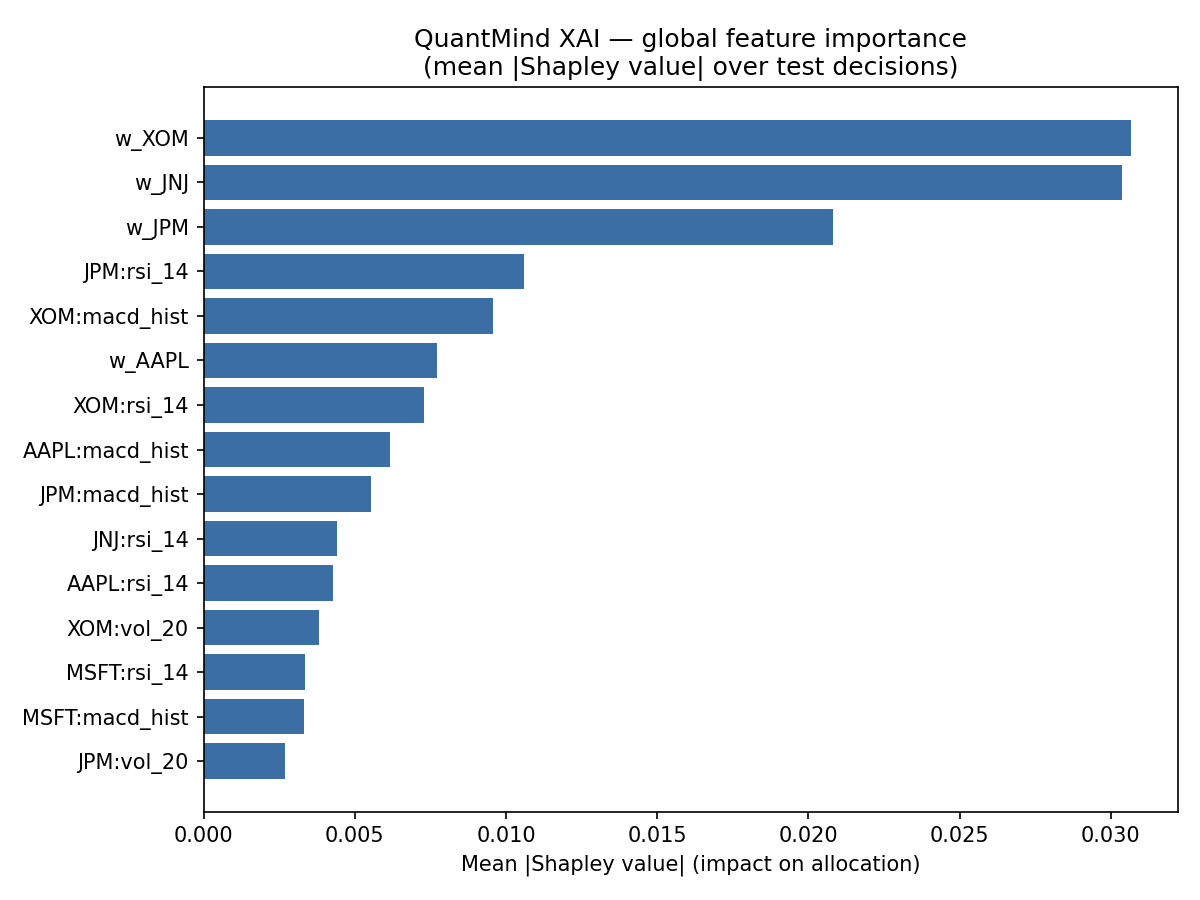
\includegraphics[width=0.68\textwidth]{figures/shap_importance.png}
\caption{Global feature importance, as the mean absolute Shapley value across test
decisions.}
\label{fig:shap}
\end{figure}

\subsection{What worked and what did not}

The prototype shows the core idea works. An RL agent can learn a steady, diversified
strategy that beats a passive baseline on risk-adjusted return out of sample. Its
choices can be explained. Building it taught me two things the hard way. An early
version reported a Sharpe ratio of about 8.5, which is not believable. The cause was
look-ahead bias: the reward used the same day's return that the agent could already
see in its features. Once I moved the reward to the next day's return, the figure
dropped to a sensible level. This is the exact trap the literature warns about. It is
easy to miss without a sanity check on the numbers. The second lesson was cost. A
plain reward made the agent trade constantly, with daily turnover near 16\%, so
trading costs ate the returns. Adding the turnover penalty and the concentration cap
fixed it and produced the behaviour in Figure~\ref{fig:alloc}.

The limits are real and worth stating plainly. A Sharpe of 0.91 is below the 1.2 I
had hoped for, so the edge over buy-and-hold is modest. The result rests on one asset
set, one test window and one random seed, so it may not hold elsewhere. The agent
also leans on a few defensive and energy names that did well in this period, which
could be a trait of the period rather than skill.

\subsection{How I would improve it}

The evaluation plan in Section 3 already names the main fixes. The prototype confirms
they are the right ones. Walk-forward testing across several windows and repeated
seeds would show how stable the result is, turning a single number into a range.
Adding the FinBERT sentiment feature is the most promising untested change, since
price data alone is a thin signal and the design already has a slot for it. A reward
built directly on a risk-adjusted measure, in the spirit of Moody and Saffell
\cite{moody2001}, might suit the goal better than the current shaped reward and cut
some of the hand-tuning. Last, the user study would test the other half of the
project: whether the Shapley-based explanations really make a non-expert more willing
to trust and act on the advice. That is the claim the whole system rests on.

\newpage
\bibliography{mybib}

\end{document}
